\section{Introduction}\label{sec:algo}
In this project, we intend to implement face detection algorithm based on the Viola Jones 
classifier ~\cite{viola_jones} on GPU. As a starting point, we take the GNU licensed C++ program that has the algorithm 
implemented to detect faces in images ~\cite{project_link}. There are various portions in the algorithm that can be 
parallelized and hence can leverage the hardware of GPU efficiently. 
Section 1 explains Viola Jones algorithm briefly. 
Section 2 explains the portions we are going to parallelize and offload to the GPU.

\section{Viola Jones Face Detection Algorithm}
The algorithm has four stages as described below
1. Haar feature selection: 
The Viola Jones classifier method is based on Haar-like features. The features consist of 
white and black rectangles as shown in Figure~\ref{fig:haar}. These features can be thought of as pixel intensity evaluation sets. 
For each feature, we subtract black region’s pixel value sum from white region’s pixel value sum. 
If this sum is greater than some threshold, it is decided that the region has this feature. 
This is the characteristic value of a feature. We have the Haar features to be used for face detection.

\begin{figure}[h]
  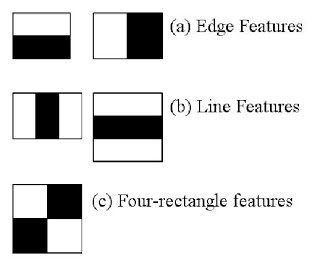
\includegraphics[width=0.45\linewidth]{figs/haar.jpg}
  \caption{Four kinds of HAAR feature rectangles \textnormal{\small }  }
  \label{fig:haar}
\end{figure}

2. Integral image: The calculation of characteristic value of a feature is an important step in 
face detection. It has to be calculated for every possible pixel region in the given image. 
In order to efficiently determine the value, integral image of the given image is used. 
For any given pixel (x, y), the integral value is the sum of all the pixels above and to 
the left of (x, y), inclusive.
i,e., If v(x’, y’) is the value of a pixel at (x’, y’), Integral Sum
IS(x, y) = x'x, y'yv(x’, y’)
Now, the sum of any given region with corner integral pixels A, B, C, D is
Sum = D+A-B-C as shown in Figure~\ref{fig:sum}.

\begin{figure}[h]
  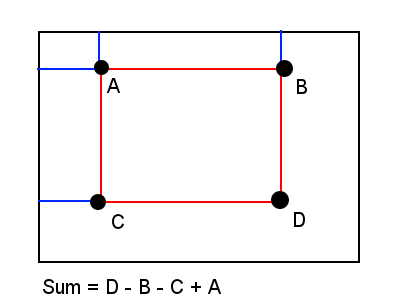
\includegraphics[width=0.45\linewidth]{figs/sum.png}
  \caption{Sum of a sub-window using Integral Image \textnormal{\small }  }
  \label{fig:sum}
\end{figure}

As shown in Figure~\ref{fig:example}, if we want to obtain the sum of 2x3 sub-window, 
integral image involves just 2 additions and 2 subtractions instead of 6 additions.

\begin{figure}[h]
  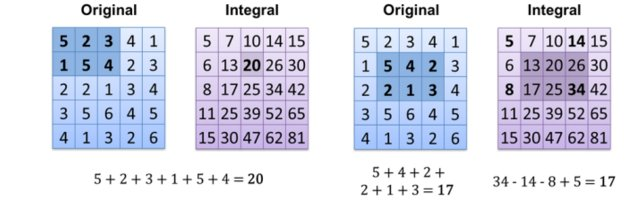
\includegraphics[width=0.45\linewidth]{figs/example.jpg}
  \caption{Example of Integral Image calculation \textnormal{\small }  }
  \label{fig:example}
\end{figure}

3. Adaboost algorithm: Adaboost or Adaptive Boosting is a machine learning algorithm 
where the output of weak classifiers is combined into a weighted sum that represents the output 
of a boosted (strong) classifier. This algorithm is used to combine features that cover facial 
characteristics to form a weak classifier. It then creates a string classifier using a group 
of weak classifiers. It further concatenates the strong classifiers to a cascade classifier.

4. Cascade classifier: A sub-window in the image that passes through the entire cascade 
classifier is detected as human face (Figure~\ref{fig:cascade}). In this project, we use 25 stages in cascade classifier. 
\begin{figure*}
  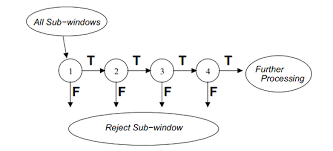
\includegraphics[width=0.9\linewidth]{figs/cascade.png}
  \caption{Cascade Classifier \textnormal{\small }  }
  \label{fig:cascade}
\end{figure}

